\chapter{PRUEBAS Y RESULTADOS}
\section{Rendimiento algoritmos de asociaci\'on}

El conjunto de datos utilizados en las pruebas pertenecen a las transacciones de uno de los supermercados m\'as 
importantes del departamento de Nari\~no (Colombia) durante un periodo determinado. El conjunto de datos contiene 
10.757 diferentes productos. Los conjuntos de datos minados con la herramienta TariyKDD se muestran en el cuadro
\ref{conjuntos}.\\
\\
Para cada conjunto de datos se realiz\'o preprocesamiento y transformaci\'on de datos con el fin de eliminar los 
productos repetidos en cada transacci\'on y posteriormente se cargaron las tablas objeto de un modelo simple
(i.e. una tabla con esquema Tid, Item) a la estructura de datos DataSet descrito en el cap\'itulo 7 en la
secci\'on de implementaci\'on.\\

\begin{table}[h]
\caption{Conjuntos de Datos}
\label{conjuntos}
\end{table}
\begin{center}
\begin{tabular}{|p{30mm}|p{30mm}|p{30mm}|p{30mm}|}\hline
\textbf{Nomenclatura} & \textbf{Numero de Registros }& \textbf{Numero de Transaccions} & \textbf{Promedio items 
por transaccion} \\ \hline
BD85KT7 & 555.123 & 85.692 & 7 \\ \hline
BD40KT5 & 194.337 & 40.256 & 5 \\ \hline
BD10KT10 & 97.824 & 10.731 & 10 \\ \hline
\end{tabular}
\end{center}

Se evalu\'o el rendimiento de los algoritmos Apriori, FP-Growth y Equipasso, comparando los tiempos de respuesta 
para diferentes soportes m\'inimos. Los resultados de la evaluaci\'on del tiempo de ejecuci\'on de estos 
algoritmos, aplicados a los conjuntos de datos BD85KT7, BD40KT5 y BD10KT10, se pueden observar en las figuras
\ref{85k1}, \ref{40k1} y \ref{10k1} respectivamente.\\
\\
En general, observando el comportamiento de los algoritmos FP-Growth y Equipasso con los diferentes conjuntos de 
datos, se puede decir que su rendimiento es similar, contrario al tiempo de ejecuci\'on  de Apriori, que se ve 
afectado significativamente a medida que se disminuye el soporte.

\begin{table}[h]
\caption{Tiempos de ejecuci\'on tabla BD85KT7}
\end{table}
\begin{center}
\begin{tabular}{|*{4}{c|}} \hline
\multicolumn{4}{|c|}{\textbf{BD85KT7}}\\ \hline\hline
\multirow{2}{*}{Soporte (\%)} & \multicolumn{3}{|c|}{Tiempo (ms)}\\ \cline{2-4}
     & Apriori & FPGrowth & EquipAsso\\ \hline
4.15 & 750 & 166 & 85\\ \hline
4.75 & 362 & 162 & 82\\ \hline
5.35 & 365 & 164 & 83\\ \hline
5.95 & 365 & 162 & 83\\ \hline
6.55 & 120 & 159 & 80\\ \hline
\end{tabular}
\end{center}

\begin{figure}[h]
\centering
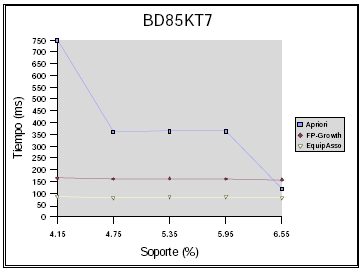
\includegraphics[width=0.7\textwidth]{images/bd85kt7.png}
\caption{Rendimiento BD85KT7}
\label{85k1}
\end{figure}

\begin{table}[h]
\caption{Tiempos de ejecuci\'on tabla BD40KT5}
\end{table}
\begin{center}
\begin{tabular}{|*{4}{c|}} \hline
\multicolumn{4}{|c|}{\textbf{BD40KT5}}\\ \hline\hline
\multirow{2}{*}{Soporte (\%)} & \multicolumn{3}{|c|}{Tiempo (ms)}\\ \cline{2-4}
     & Apriori & FPGrowth & EquipAsso\\ \hline
1.90 & 268 & 66 & 29\\ \hline
2.00 & 265 & 64 & 29\\ \hline
2.10 & 132 & 63 & 27\\ \hline
2.20 &  45 & 61 & 27\\ \hline
2.30 &  44 & 61 & 27\\ \hline
\end{tabular}
\end{center}

\begin{figure}[h]
\centering
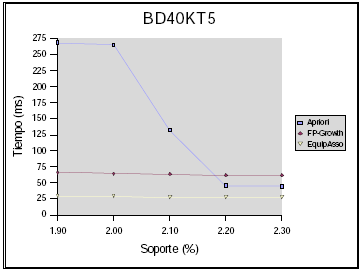
\includegraphics[width=0.7\textwidth]{images/bd40kt5.png}
\caption{Rendimiento BD40KT5}
\label{40k1}
\end{figure}

\newpage

\begin{table}[h]
\caption{Tiempos de ejecuci\'on tabla BD10KT10}
\end{table}
\begin{center}
\begin{tabular}{|*{4}{c|}} \hline
\multicolumn{4}{|c|}{\textbf{BD10KT10}}\\ \hline\hline
\multirow{2}{*}{Soporte (\%)} & \multicolumn{3}{|c|}{Tiempo (ms)}\\ \cline{2-4}
     & Apriori & FPGrowth & EquipAsso\\ \hline
3.00 & 525 & 28 & 15\\ \hline
4.00 & 182 & 26 & 14\\ \hline
5.00 & 105 & 25 & 13\\ \hline
6.00 &  53 & 24 & 13\\ \hline
7.00 &  52 & 24 & 13\\ \hline
\end{tabular}
\end{center}

\begin{figure}[h]
\centering
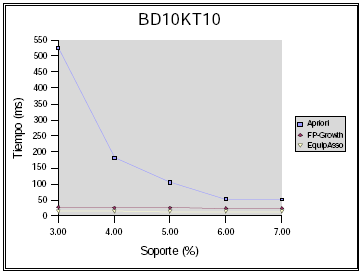
\includegraphics[width=0.7\textwidth]{images/bd10kt10.png}
\caption{Rendimiento BD10KT10}
\label{10k1}
\end{figure}

\newpage

Analizando el tiempo de ejecuci\'on de \'unicamente los algoritmos FP-Growth y EquipAsso (figuras \ref{85k2}, 
\ref{40k2} y \ref{10k2}) para los conjuntos de datos BD85KT7, BD40KT5 y BD10KT10. Con soportes m\'as bajos, el
comportamiento de estos algoritmos sigue siendo similar.

\begin{table}[h]
\caption{Tiempos de ejecuci\'on tabla BD85KT7}
\end{table}
\begin{center}
\begin{tabular}{|*{4}{c|}} \hline
\multicolumn{4}{|c|}{\textbf{BD85KT7}}\\ \hline\hline
\multirow{2}{*}{Soporte (\%)} & \multicolumn{3}{|c|}{Tiempo (ms)}\\ \cline{2-4}
     & Apriori & FPGrowth & EquipAsso\\ \hline
1.00 & - & 5130 & 1225\\ \hline
1.50 & - &  730 & 270\\ \hline
2.00 & - &  212 & 205\\ \hline
2.50 & - &  202 & 202\\ \hline
3.00 & - &  185 & 187\\ \hline
\end{tabular}
\end{center}

\begin{figure}[h]
\centering
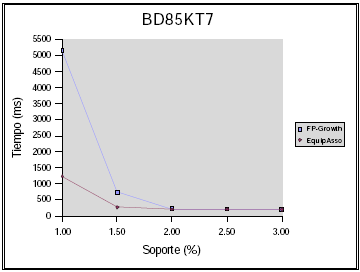
\includegraphics[width=0.7\textwidth]{images/bd85kt72.png}
\caption{Rendimiento BD85KT7}
\label{85k2}
\end{figure}

\begin{table}[h]
\caption{Tiempos de ejecuci\'on tabla BD40KT5}
\end{table}
\begin{center}
\begin{tabular}{|*{4}{c|}} \hline
\multicolumn{4}{|c|}{\textbf{BD40KT5}}\\ \hline\hline
\multirow{2}{*}{Soporte (\%)} & \multicolumn{3}{|c|}{Tiempo (ms)}\\ \cline{2-4}
     & Apriori & FPGrowth & EquipAsso\\ \hline
0.10 & - & 965 & 741\\ \hline
0.20 & - & 425 & 290\\ \hline
0.30 & - & 240 & 168\\ \hline
0.40 & - & 156 & 121\\ \hline
0.50 & - & 124 & 105\\ \hline
\end{tabular}
\end{center}

\begin{figure}[h]
\centering
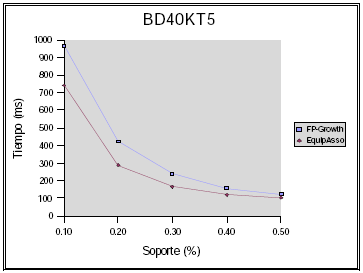
\includegraphics[width=0.7\textwidth]{images/bd40kt52.png}
\caption{Rendimiento BD40KT5}
\label{40k2}
\end{figure}

\newpage

\begin{table}[h]
\caption{Tiempos de ejecuci\'on tabla BD10KT10}
\end{table}
\begin{center}
\begin{tabular}{|*{4}{c|}} \hline
\multicolumn{4}{|c|}{\textbf{BD10KT10}}\\ \hline\hline
\multirow{2}{*}{Soporte (\%)} & \multicolumn{3}{|c|}{Tiempo (ms)}\\ \cline{2-4}
     & Apriori & FPGrowth & EquipAsso\\ \hline
0.50 & - & 257 & 181\\ \hline
0.75 & - & 133 & 93\\ \hline
1.00 & - &  78 & 60\\ \hline
1.25 & - &  61 & 50\\ \hline
1.50 & - &  46 & 42\\ \hline
\end{tabular}
\end{center}

\begin{figure}[h]
\centering
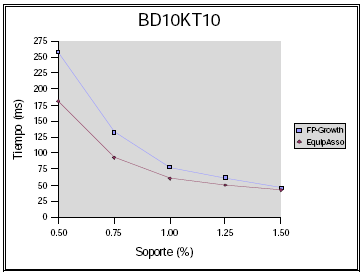
\includegraphics[width=0.7\textwidth]{images/bd10kt102.png}
\caption{Rendimiento BD10KT10}
\label{10k2}
\end{figure}

